\section{Background}

\subsection{Usage Scenario}
\subsubsection{Student}
\textbf{User Story: I have just started the course and I want to find more information about my lectures and assignments.}
\begin{itemize}
    \item{I log in to the student portal with my name or student number}
    \item{I ask the bot questions:}
    \begin{itemize}
        \item{Who is the lecturer? \textit{“John Shepherd lecturer”}}
        \item{When is my assignment due? \textit{“Assignment 1 submission week 6 worth 9, assignment 2 submission week 10 worth 11”}}
        \item{How do I do the labs? \textit{“Each week there will be one or more exercises to work on. These exercises will be released in the week preceding the lab class. Labs will be done in pairs and you and your lab partner should discuss the exercises before going to the lab to maximise the usefulness of the class...”}}
    \end{itemize}
\end{itemize}

\textbf{User Story: I have some questions for COMP1521 that I want the answer to right away. It’s a few days until my next tutorial.}
\begin{itemize}
    \item{I log in again}
    \item{I ask the bot questions:}
    \begin{itemize}
        \item{What is qtspim? \textit{“Qtspim... provides a gui front-end useful for debugging”}}
        \item{How do I make a stack frame in MIPS? \textit{“Create a stack frame for itself change \$fp and \$sp. Save the return address \$ra in the stack frame. Save and \$s registers that it plans to change”}}
        \item{What are the MIPS floating point registers? \textit{“Mips has 32 32-bit general purpose registers and 16 64-bit floating point registers as well as two special registers hi and lo for manipulating 64-bit integer quantities...”}}
        \item{What is the clock sweep algorithm? \textit{“Uses a reference bit for each frame updated when page is used. Maintains a circular list of allocated frames. Uses a clock hand which iterated over page frame list skipping and resetting reference bit in all reference pages...”}}
        \item{What does execve do? \textit{“Execve... Convert one process into another”}}
        \item{What is envp? \textit{“Envp contains strings of the form key-value”}}
        \item{What does fork do? \textit{“Fork... Create a new child process copy of current process”}}
        \item{What does sigpipe mean? \textit{“Sigpipe... broken pipe no processes reading from pipe”}}
        \item{What does sighup mean? \textit{“Sighup... hangup detected on controlling terminal/process”}}
    \end{itemize}
    \item{I get these answers right away and don’t have to ask my tutor.}
\end{itemize}

\newpage
\textbf{User Story: I want to revise for the midterm test.}
\begin{itemize}
    \item{I log in to the chat bot and ask “quiz me”}
    \item{I read the quiz questions and try to answer them}
    \item{I click “show answer” and check if my answer was right or not}
    \item{I am having difficulty with the revision questions for process management in C, so I ask “quiz me on C process management”}
    \item{I get some quiz questions specifically about that topic}
    \begin{itemize}
        \item{\textit{What happens to a child process if the parent process exits?}}
    \end{itemize}
    \item{I think about the answer and once I decide, I check if I was correct by clicking “show answer”, which displays the admin inputted data}
\end{itemize}

\subsubsection{Course Administrator}
\textbf{User Story: I want to set up my course to work with the chat bot, so that my students can use it.}
\begin{itemize}
    \item{I register and log in to the admin portal}
    \item{I input my course information in the new course setup page}
    \item{I supply links to the html pages I want to be included in the data: course outline, assignment specifications, and course content pages that are available online}
    \item{I submit the form, and then when the course setup is ready, I’ll be able to see it in the admin portal when I refresh the page}
    \item{The setup might take a few minutes as the data is processed, but I can do something else while I wait}
\end{itemize}

\textbf{User Story: I want to add quiz questions for my course to help my students revise.}
\begin{itemize}
    \item{I log in to the admin portal and select my course from the menu}
    \item{I view the quiz questions I have already added}
    \item{I delete some old questions I no longer want my students to see}
    \item{I select “add questions” and input more questions}
    \begin{itemize}
        \item{What is the size of the general registers in MIPS? Why can’t we store a C long long int, in the \$t0 register? \textit{mips is a 32 bit architecture and as such the registers and relevant logic circuits only support 32 bit numbers.}}
        \item{What happens to a child process if the parent process exits? \textit{The child process runs independently and does not exit.}}
    \end{itemize}
    \item{These will be available right away to students}
\end{itemize}

\subsection{System Architecture}
\subsubsection{Architecture Diagram}
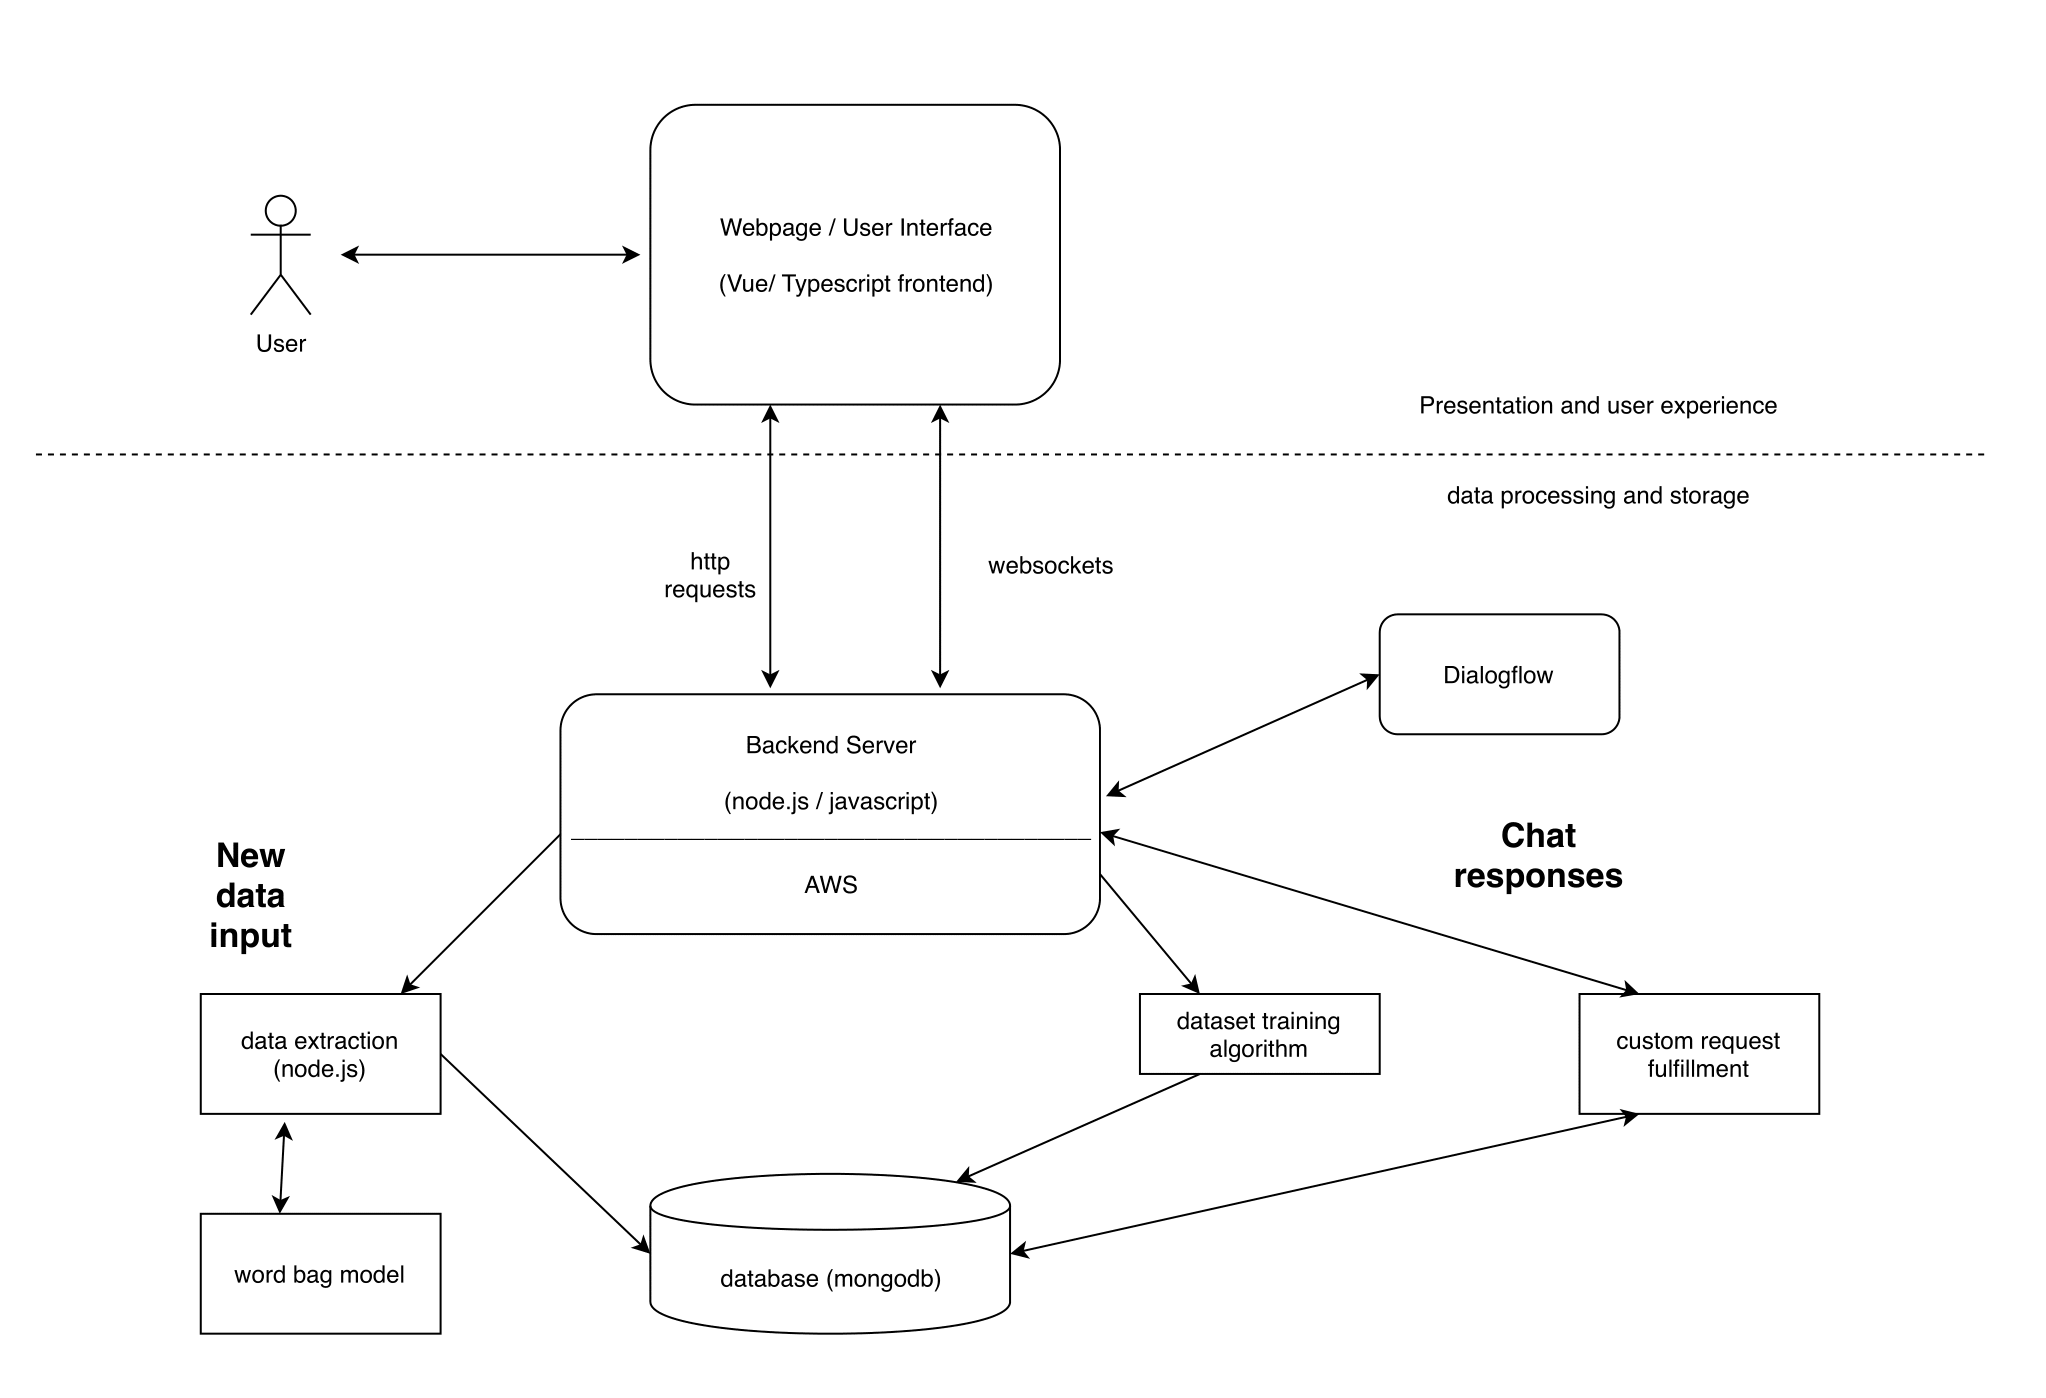
\includegraphics[width=\textwidth]{architecture-diagram.png}

\subsubsection{Data Scraping \& Processing}

\subsubsection{Extensible Backend}
% Our bot was built entirely from scratch, with limited dependency on external APIs. We have constructed a backend in \code{Javascript} using \code{Node.js}. This runs on an \code{EC2} instance on Amazon Web Services (AWS). The backend is responsible for a number of tasks, including but not limited to processing user queries, generating intelligent responses, managing user sessions and providing access to the relevant databases for user accounts and quiz questions.

% We also developed a web frontend for our bot using \code{Vue.js}. 

\subsubsection{Interactive User Interface}

\newpage
